\begin{frame}
	{Shifting gears \& talk about how to talk to the devices}

	But the real advantage to IoT is the I - Internet!

	Lots of good ways to do this...

	\begin{multicols}{2}
		\begin{small}
		\begin{multicols}{2}
			\begin{itemize}
				\item MQTT
				\item Liota
				\item AMQP
				\item STOMP
				\item RabbitMQ
				\item REST
				\item WAMP
				\item ZeroMQ
				\item Java Message\linebreak Service (JMS)
				\item CoAP
				\item CLOUD!
				\item XMPP-IOT
				\item XMPP
				\item etc...
			\end{itemize}
		\end{multicols}
		\end{small}

		\vfill\null
		\columnbreak

		\begin{figure}[H]
			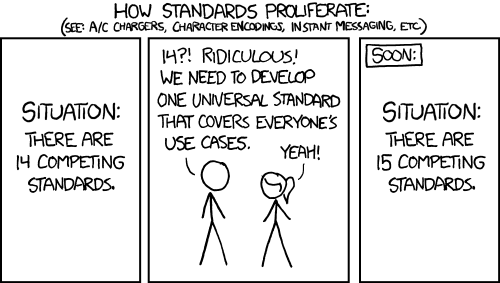
\includegraphics[width=0.95\linewidth]{IMAGES/XKCD_Standards}
			\captionsetup{labelformat=empty}
			\caption{
				{\scriptsize\url{https://xkcd.com/927/} - CC-BY-NC 2.5}
			}
		\end{figure}
	\end{multicols}

\end{frame}

\cprotect\note{
	% Speaker notes go here
}

% vim:colorcolumn=80:display+=lastline:linebreak:wrap:tw=80:tabstop=4:shiftwidth=4
